\documentclass[a4paper,12pt]{article}

\usepackage[utf8]{inputenc}
\usepackage[english]{babel}
\usepackage{algorithm}
\usepackage{comment}
\usepackage{amssymb,amsmath,amsthm}
\usepackage{graphicx}

% set the theorem styles according to the argument
\newtheorem{theorem}{Theorem}[section]
\newtheorem{lemma}[theorem]{Lemma}
\newtheorem{assumption}[theorem]{Assumption}
\newtheorem{definition}[theorem]{Definition}


\begin{document}

\begin{abstract}

Modern digital services need ML pipelines that learn, unlearn, and predict continously. Models need to learn on production data streams, adapting to changing and nonstationary environments. We introduce a memory pair framework that pairs the learning and unlearning processes into a single developer-friendy API. The algorithm handles a stream of interleaved \texttt{insert}, \texttt{delete}, and \texttt{predict} events and processes them sequentially with $(\epsilon, \delta)$-certified unlearning. Using an online variant of L-BFGS, we're able to achieve sublinear cumulative regret for the entire stream of deletions up to the theoretically-derived capacity bound. A lightweight odometer is used to track the deletion capacity of the model to ensure performance guarantees.

\end{abstract}


\section{Introduction}
\label{sec:intro}

Industry has transitioned to a serverless and event-based cloud architecture for software. State changes are communicated with ACID transactions that contain as much information as the data store itself. Developers need stream-native learners that can learn continuously while performing inference.

The problem is made more interesting by recent legislation. The European Union's General Data Protection Regulation provides users the right to be forgotten: to have their data summarily deleted from a company's servers, and the effect of such data removed from a statistical model.

We provide a framework for online algorithms that encompasses both learning and unlearning. We build specifically for the case of distributed systems where learning and unlearning are \textbf{necessary, interleaved} operations used to refine model accuracy. We show that the memory pair meets state of the art regret guarantees with a sublinear memory footprint particularly suited for online learning. It also satisfies $(\epsilon,\delta)$-unlearning requirements, which makes it particularly suitable for the task of machine learning.

Machine unlearning research has begun to address the privacy side.  The frameworks of Sekhari et al. and Qiao et al. provide provable $(\varepsilon,\delta)$ guarantees that a post-hoc deletion yields (in distribution) the same parameters as a fresh retrain.  However, both assume an offline model that never learns again after deletion. We assume a stream environment where distributions drift continuously, and we show that our model adapts to such environments while preserving performance.

\section{Stream-Native Learning}
\label{sec:stream-native}

The next generation of ML systems must treat \textit{learning}, \textit{forgetting}, and \textit{predicting} as first-class, intertwined operations performed on a live data stream.  To this end we introduce the \textbf{Memory Pair} pipeline:

\begin{itemize}
    \item \textit{Stream-native learning:} A learner $A$ ingests each example $(x_t,y_t)$ and performs an $O(d)$ update in micro-seconds, maintaining only lightweight sketches instead of per-sample gradients.
    \item \textit{Deferred inference gate:} Predictions are withheld until the running sample count exceeds a theoretically derived sample-complexity threshold, ensuring the first answer is already PAC-competitive.
    \item \textit{Symmetric unlearning:} A paired algorithm $\bar{A}$ accepts deletion requests via the same API and issues a one-step \textit{negative} update that preserves the learner’s regret bound. The model is guaranteed to be within an arbitrary precision of the ideal cold-start model trained from scratch.
    \item \textit{Live deletion-capacity odometer:} Each unlearning step depletes the model's deletion capacity budget. When a model unlearns its capacity, the learner is flagged for retraining to preserve accuracy. We ensure tight accounting on model capacity to not only take models down on time, but to stretch the duration of a model's reliability.
\end{itemize}

\subsection{Contributions}

The batch unlearning framework from Sekhari et al. provides the theoretical inspiration for true online unlearning. By focusing on population risk, they establish that unlearning with generalization guarantees is possible. However, their algorithm is designed for a static, i.i.d. world.

Our Memory Pair framework adapts these core ideas for a dynamic, online setting. We replace the assumption of i.i.d. data with a non-stationary stream, substitute the excess risk metric with the more robust notion of cumulative regret, and swap the expensive, offline Hessian-based update with a lightweight, stream-native L-BFGS approximation. 

The Memory Pair is not just a generalization of the batch algorithm but a \textit{necessary evolution} designed to handle the continuous learning, forgetting, and inference demands of a live data stream.

\section{Preliminaries}
\label{sec:prelim}

We start by framing our learners within the online learning paradigm. Batch learning  minimizes the loss function evaluated over a static training set. We instead use the seminal notion of regret, which appropriately compares the online learner to the best possible model in hindsight for a particular realized sequence of events.

This demonstrates the key factor of the Sekhari paper. By requiring the model to satisfy population risk guarantees, the model is expected to perform well against some true but unknown parameter distribution. This is very similar to the case of online learning because the model's evaluation is continuous, and the descent is adjusted accordingly.

\begin{definition}[Online learner with vanishing average regret]
\label{def:online-learner}
Let $\mathcal W \subseteq \mathbb{R}^d$ be a convex hypothesis set and $\{\ell_t\}_{t=1}^\infty$ an arbitrary sequence of (not necessarily stationary) loss functions $\ell_t : \mathcal W \to \mathbb{R}_{\ge 0}$. An algorithm $\mathcal A$ that, after observing an outcome $(x_t,y_t)$, outputs a weight vector $w_t = \mathcal A(x_{1:t},y_{1:t}) \in \mathcal W$ is called an \emph{online learner} iff for every outcome sequence $\{(x_t,y_t)\}_{t=1}^\infty$ the \emph{average regret}
\[
  \frac{1}{n}\,R_n(\mathcal A)
  \;:=\;
  \frac{1}{n}
  \Bigl(
    \sum_{t=1}^{n}\ell_t(w_t)
    -
    \min_{w\in\mathcal W}\sum_{t=1}^{n}\ell_t(w)
  \Bigr)
\]
converges to zero,
i.e.
\[
  \frac{1}{n}\,R_n(\mathcal A)
  \;\xrightarrow[n\to\infty]{}\;0.
\]
\end{definition}

In the online setting, a model is expected not only to learn incrementally, but also process data deletion requests with some measure of guarantee. The unlearning algorithm must yield a model that is statistically indistinguishable from the model's ideal state: a model trained from scratch without the offending data. This tight, state-dependent relationship requires a unified framework where learning and unlearning procedures are tightly coupled.

We formalize the notion of a memory pair as a coupled learning-unlearning algorithm designed to operate on a stream of insertions and deletions. A valid memory pair must simultaneously guarantee learning accuracy constraints, unlearning fidelity, and the capacity to handle a certain number of deletions.

\begin{definition}[Memory Pair]
\label{def:memory-pair}

Let $\{E\}_{t=1}^{N}$ be an event stream where $E_{t} \in \{\text{insert}(x_{t},y_{t}), \text{delete}(u_{t})\}$. A pair of algorithms $(A, \bar{A})$ with shared state $\theta_{t-1}$ acts as follows:

$$
\text{learn step: }\theta_t = A(\theta_{t-1},E_t) 
$$
$$
\text{unlearn step: } \bar{\theta_{t}} = \bar{A}(\theta_{t-1},E_{t})
$$

Denote by $\tilde \theta_{t}$ the ideal replay model: the model state achieved by processing all \textsc{insert} events up to time $t$ except those whose index has appeared in a prior \textsc{delete} event. Fix an accuracy target $\gamma$, confidence $\delta$, privacy budget $(\varepsilon^{\star},\delta^{\star})$, and deletion capacity $m$. Then $(A,\bar A)$ is a \emph{$(\gamma,m,\varepsilon^{\star},\delta^{\star})$-memory pair} if the following hold for every event stream and for all horizons $N$:

\begin{enumerate}
\item \textbf{Online accuracy.} The average regret over the realized stream satisfies

\[
\Pr\!\bigl[\tfrac{1}{N} R_N(\theta)\le\gamma\bigr] \;\ge\; 1-\delta.
\]

\item \textbf{$(\varepsilon,\delta)$-Online Unlearning.} For every measurable set $S\subseteq\mathcal W$ and every time $t\!\le\!N$, the unlearned model $\bar\theta_{t}$ is $(\varepsilon^{\star},\delta^{\star})$-indistinguishable from the ideal replay model $\tilde\theta_{t}$:
\[
    \Pr[\tilde\theta_t\in S] \le e^{\varepsilon^\star}\Pr[\bar\theta_t\in S]+\delta^\star \quad \text{and} \quad \Pr[\bar\theta_t\in S] \le e^{\varepsilon^\star}\Pr[\tilde\theta_t\in S]+\delta^\star.
\]

\item \textbf{m-deletion capacity.} Let $D_N$ be the number of \textsc{delete} events up to $N$. If $D_N\le m$, then Conditions (I) and (II) hold.

\end{enumerate}
\end{definition}

The memory pair definition allows for interleaved insert, delete, and predict operations. It combines the accuracy guarantees of learning algorithms with the certifiable unlearning guarantees that are ubiquitous in machine unlearning. Bundling the learning and unlearning algorithms is a natural extension to a body of work that has increasingly found them inseparable. Indeed, recent Hessian-free methods of machine unlearning explicitly use the learning process to gain gradient information that is later used to unlearn.

\subsection{Related Work}

This algorithm is inspired by the Newton Step algorithm for certifiable machine unlearning from Sekhari et al. The seminal paper demonstrates the inherent difficulty of the unlearning problem when minimizing population risk. They derive the nontrivial bound of deletion capacity if the learner is to perform well in production. Specifically, the notion that performance should generalize for points not yet seen by the model.

There is a very natural relationship between performing well on an unseen test dataset and performing well on a sequence of incrementally-revealed stream events in the online setting. We build on Sekhari et al.'s initial work by pairing the learning and unlearning processes into a single framework, expanding performance guarantees to the online case, and providing online generalizations of the notions of sample complexity and deletion capacity. We additionally replace the expensive Hessian inversion with an online variant of L-BFGS that removes the linearly-scaled memory footprint.

\section{Memory Pair}
\label{sec:memory-pair}

\subsection{Newton-Step Approach to Machine Unlearning}

Machine unlearning has a rich tool set of algorithms to approximate the ideal retrained model. One of the strongest is Sekhari et al.'s application of the Newton Step optimization method to remove the influence of a set of unlearned points. With careful noise calibration, the unlearned method is certifiably indistinguishable from the ideal cold-start retrained model.

The unlearning approximation draws its strength from the second-order information of the model's training curve stored in the Hessian. Scaling our average loss by the the inverse Hessian allows us to approximate the impact of those unlearned points on the model's parameters in the form of a model update. A small amount of calibrated noise is then added to those weights to ensure certifiable indistinguishability from the retrained model. But with an $O(d^{2})$ runtime complexity, the option is not computationally efficient.

There has also been recent work into Hessian-Free unlearning, which stores gradient approximations of the training data to create a suitable estimate of the inverse Hessian using Hessian Vector Products. But with a memory footprint that scales linearly, it is not feasible for the online use case where $n>>d$.

\subsection{Quasi-Newton Approaches to Online Learning}

We specifically target the Hessian inversion operation of the Newton-Step update for our unlearning algorithm. We replace the Hessian inversion with an online variant of the L-BFGS optimization algorithm. This eliminates the need for the precomputation stage present in Hessian-Free and standard Newton Step unlearning. In fact, it enables a broader prediction space entirely. With no precompute required for deletion, interleaved learning and unlearning operations can be processed sequentially as the events are read from a data stream. This is especially attractive for the prospect of federated learning with on-device learning. More on this in Future Work.

The method efficiently updates the gradient near-instantaneously by computing the current gradient with respect to the point. The curvature points from the L-BFGS are then used to approximate something like a Hessian inversion. The key is to use the second-order curvature information from the saved points to approximate the curvature of the whole function.

When the curvature points are used to approximate the second-order information for a whole function, the choice of points holds some weight. The online variant of L-BFGS is used for precisely this reason, easily ingesting and disposing of curvature points as additional information is fed through the insertion operations.

\begin{algorithm}
\caption{Memory Pair Insertion}\label{alg:insertion}
\begin{algorithmic}
\Require New data point $(x, y)$, Model state $(\theta, \text{lbfgs})$
\State $g_{\text{old}} \gets \nabla_{\theta} \mathcal{L}(\theta; x, y)$
\Comment{Compute gradient at current parameters}
\State $d \gets \text{lbfgs.direction}(g_{\text{old}})$
\Comment{Compute quasi-Newton direction}
\State $\theta_{\text{new}} \gets \theta + \alpha d$
\Comment{Update parameters with learning rate $\alpha$}
\State
\State $s \gets \theta_{\text{new}} - \theta$
\Comment{Compute change in parameters}
\State $\theta \gets \theta_{\text{new}}$
\Comment{Commit the parameter update}
\State $g_{\text{new}} \gets \nabla_{\theta} \mathcal{L}(\theta; x, y)$
\Comment{Compute gradient at new parameters}
\State $y_{\text{vec}} \gets g_{\text{new}} - g_{\text{old}}$
\Comment{Compute change in gradient}
\State
\State $\text{lbfgs.add\_pair}(s, y_{\text{vec}})$
\Comment{Update L-BFGS curvature memory}
\end{algorithmic}
\end{algorithm}

The deletion method works by computing the unlearned point's gradient using the model's learned parameters. The influence of the point is approximated using the L-BFGS approximation and used in place of the explicitly calculated inverse Hessian in typical Newton methods. 

Before the weight parameter is returned, there is a calibrated amount of noise added to the estimate. This amount of noise serves two purposes: (1) differential privacy with respect to the unlearned data and (2) blurring the remaining difference between the unlearned model and the ideal cold-start. Too little noise will violate the indistinguishability requirement for the incrementally unlearned model from the ideal retrain. Too much noise will violate our regret convergence guarantees.

When chosen carefully, the noise acts as a shock absorber for the model. It dampens the unlearning effect that would leak the deleted user's information. Our variance is specifically chosen to outpace both the (1) Hessian-sketch error of L-BFGS and (2) the cumulative impact of all future deletions. We can estimate the second because we explicitly limit the number of deletions with deletion capacity and ensure its compliance with our capacity odometer.

The unlearning algorithm is defined analogously. It takes the point to be deleted and computes the gradient of the loss at the point of prediction. The L-BFGS method is used to estimate the influence of that point on the historical trajectory of the algorithm (approximated using the curvature points) to estimate the same Hessian inversion performed by the Newton Step.

\begin{algorithm}
\caption{Memory Pair Deletion}\label{alg:deletion}
\begin{algorithmic}
\Require Data point to delete $(x, y)$, Model state $(\theta, \text{lbfgs})$, Budgets $(\epsilon_{\text{step}}, \delta_{\text{step}})$
\If{$\text{deletions\_so\_far} \geq K$ \textbf{or} len(lbfgs) == 0}
\State \textbf{raise} RuntimeError
\EndIf
\State
\State $g \gets \nabla_{\theta} \mathcal{L}(\theta; x, y)$
\Comment{Compute gradient of the point to unlearn}
\State $d \gets \text{lbfgs.direction}(g)$
\State $\theta \gets \theta - d$
\Comment{Remove the approximate influence}
\State
\State $\text{sensitivity} \gets \|d\|_2$
\State $\sigma \gets \frac{\text{sensitivity} \cdot \sqrt{2 \ln(1.25 / \delta_{\text{step}})}}{\epsilon_{\text{step}}}$
\Comment{Calibrate noise}
\State $\eta \sim \mathcal{N}(0, \sigma^2 I_d)$
\State $\theta \gets \theta + \eta$
\Comment{Inject noise to ensure unlearning guarantee}
\State
\State $\epsilon_{\text{spent}} \gets \epsilon_{\text{spent}} + \epsilon_{\text{step}}$
\Comment{Update privacy odometer}
\State $\text{deletions\_so\_far} \gets \text{deletions\_so\_far} + 1$

\end{algorithmic}
\end{algorithm}

\subsection{Privacy Accounting via a Deletion Odometer}

A critical component of the Memory Pair framework is its ability to manage the trade-off between unlearning fidelity and model accuracy. This is accomplished through a strict accounting mechanism that we term a \textbf{privacy odometer}. Unlike a dynamic process where capacity might change, our framework treats the privacy budget as a finite resource that is determined at initialization and consumed with each deletion request.

The model is initialized with a fixed \textbf{m-deletion capacity}, corresponding to the \texttt{max\_deletions} parameter, which represents the total number of unlearning operations the model can perform before its guarantees are void. The total privacy budget, $(\epsilon_{\text{total}}, \delta_{\text{total}})$, is apportioned uniformly across this capacity. The per-step budget for each deletion is therefore:
$$
\epsilon_{\text{step}} = \frac{\epsilon_{\text{total}}}{2 \cdot m} \quad \text{and} \quad \delta_{\text{step}} = \frac{\delta_{\text{total}}}{2 \cdot m}
$$
This apportionment ensures that the cumulative privacy loss remains bounded after the model has serviced all $m$ deletion requests.

The framework acts as accountant by tracking two metrics: \texttt{deletions\_so\_far} and \texttt{eps\_spent}. When a \texttt{delete} operation is called, the accountant first checks if the capacity has been exceeded. If \texttt{deletions\_so\_far} has reached $m$, a \texttt{RuntimeError} is raised, halting further unlearning and signaling that the model must be retrained from scratch to preserve its integrity.

This finite capacity is not an arbitrary limitation but a necessary consequence of the inherent tension between privacy and accuracy. Each deletion operation injects calibrated noise into the model's parameters to satisfy the $(\epsilon, \delta)$-unlearning guarantee. While a single injection has a negligible effect, the cumulative impact of this noise degrades model accuracy. The $m$-deletion capacity thus represents the maximum number of deletions the model can sustain while ensuring that the cumulative noise does not overwhelm the learning signal and violate the learner's average regret bound, $\gamma$.

\section{Theoretical Evaluation}
\label{sec:theory}

The move from batch to stochastic setting is made easier by Sekhari et al.'s  proof of an unlearning algorithm with guaranteed performance on unseen data. Such a tool wonderfully translates the stochastic notion of population risk to the online notion of regret. While population risk measures the model's performance against a static underlying dataset, cumulative regret evaluates our learner against the \textit{best static model in hindsight for the specific, realized sequence of data}.

Our goal becomes more complex because of the optimizations used to approximate the Hessian. We first establish the sensitivity of a deletion performed using online L-BFGS before using that information to ensure the unlearned model is private.

\subsection{Analyzing the Impact of a Single Deletion}

We first analyze the impact of a single \textsc{delete} operation on the model's state. We use the convexity assumptions that are common in linear optimization to derive a bound in terms of the strength of the convexity assumption, $\lambda$, and the number of parameters, $L$.

\begin{assumption}[L-Bounded Gradients]
\label{assum:lipschitz}
The loss function $\mathcal{L}(\theta; z) = \frac{1}{2}(\theta^T x - y)^2$ has L-bounded gradients for any data point $z$. For $g = \nabla_\theta \mathcal{L}(\theta; z)$, we assume $||g||_2 \leq L$.
\end{assumption}

\begin{assumption}[Stable L-BFGS Approximation]
\label{assum:stable-lbfgs}
The online L-BFGS procedure maintains an inverse Hessian approximation, $B^{-1}$, whose spectral norm is bounded. This reflects the $\lambda$-strong convexity of the learning problem, such that $||B^{-1}||_2 \leq 1/\lambda$.
\end{assumption}

\begin{lemma}[Influence of a Single Deletion]
\label{lem:bounded-influence}
For a deletion operation on a data point $z=(x, y)$, let the influence direction be $d$. Under Assumptions A and B, the L2-norm of the influence direction is bounded such that:
$$
||d||_2 \leq \frac{L}{\lambda}
$$
\end{lemma}

The key is in the calibration. We use the upper bound of the norm of the step direction to indicate the worst-case of a single deletion. We're then able to carefully calibrate the noise in our Gaussian Mechanism to blur the effect of the deletion itself. This ensures that the deletion of one point is statistically indistinguishable from that of another, and prevents adversarial information leakage.

\begin{theorem}[Single‑step $(\varepsilon,\delta)$‑unlearning]
\label{thm:single-step-unlearning}
If noise $\eta\sim\mathcal N(0,\sigma^2 I)$ with  
$\sigma \ge \frac{(L/\lambda)\sqrt{2\ln(1.25/\delta)}}{\varepsilon}$  
is added as in Algorithm \ref{alg:deletion}, the update
$\bar\theta=\theta-d+\eta$ satisfies $(\varepsilon,\delta)$‑unlearning.
\end{theorem}

Since we've bound the largest possible impact from a single deletion, we're able to generalize to a stream of up to $m$ valid deletions. We bound the strength of our noise to the sensitivity of the delete operation to ensure the injected noise doesn't degrade model performance.
\subsection{Analyzing Cumulative Performance Over a Stream}

\begin{theorem}[Stream‑wide privacy \& regret guarantee]
\label{thm:comp-privacy-regret}
Fix a privacy target $(\varepsilon^{\star},\delta^{\star})\in(0,1]^{2}$ and a maximum deletion capacity $m\in\mathbb{N}$. Let the memory pair $(A,\bar A)$ operate on a stream of $T$ events that contains at most $m$ delete requests. During the $j^{\text{th}}$ delete ($1\le j\le m$) the unlearning routine

\begin{enumerate}
    \item computes the influence vector $d_{j} = -B_{t_{j}}^{-1}\nabla \ell_{t_{j}}(w_{t_{j}})$, which is bounded by Lemma~\ref{assum:lipschitz}
    \item adds Gaussian noise $\eta_j\sim\mathcal N\!\bigl(0,\sigma_{\text{step}}^2\mathbf I_d\bigr)$ with 
    \[
    \sigma_{\text{step}}^2
    \;=\;
    \Bigl(\tfrac{L}{\lambda}\Bigr)^2
    \frac{2\ln\!\bigl(1.25/\delta_{\text{step}}\bigr)}%
         {\varepsilon_{\text{step}}^{\,2}},
    \qquad
    \varepsilon_{\text{step}}:=\frac{\varepsilon^\star}{m},
    \quad
    \delta_{\text{step}}:=\frac{\delta^\star}{m},
  \]
    and sets $w_{t_j}^{\text{new}} = w_{t_j}-d_j+\eta_j$
\end{enumerate}

Then, for \emph{any} sequence of at most $m$ deletions and \emph{any}
adversarially chosen stream of $T$ loss functions
$\{\ell_t\}_{t=1}^{T}$ that satisfy Assumption~\ref{assum:lipschitz},

\begin{enumerate}
\item \textbf{Privacy / unlearning.}  
      The entire weight sequence $\{w_t^{\text{new}}\}_{t=1}^{T}$
      is $(\varepsilon^\star,\delta^\star)$‑indistinguishable
      from the ideal replay sequence
      $\{\tilde w_t\}_{t=1}^{T}$ in the sense of
      Definition~\ref{def:memory-pair}\,(II).

\item \textbf{Utility / regret.}  
      With probability at least
      $1-\delta^\star-\delta_{\mathrm{B}}$ (for an arbitrary
      $\delta_{\mathrm{B}}\!\in\!(0,1)$),
      the cumulative regret against the best fixed comparator
      $w^\star\in\arg\min_{w\in\mathcal W}\sum_{t=1}^{T}\ell_t(w)$ obeys
      \[
        R_T
        \;=\;
        \sum_{t=1}^{T}\bigl[\ell_t(w_t^{\text{new}})-\ell_t(w^\star)\bigr]
        \;\le\;
        GD\sqrt{cCT}
        \;+\;
        \frac{mL}{\lambda}\;
        \sqrt{\frac{2\ln\!\bigl(1.25m/\delta^\star\bigr)}%
                   {\varepsilon^\star}}\;
        \sqrt{2\ln(1/\delta_{\mathrm{B}})},
      \]
      where the first term is the deterministic
      $\tilde O\!\bigl(\sqrt{T}\bigr)$ bound from
      Theorem~\ref{thm:regret-lbfgs} and the second term captures the
      additional loss incurred by the injected noise.
      Consequently, $R_T = O\!\bigl(\sqrt{T}\bigr)$ as
      $T\!\to\!\infty$.
\end{enumerate}
\end{theorem}

\begin{proof}
\textbf{(i) Privacy.}
Each deletion step is a Gaussian mechanism whose $(\varepsilon_{\text{step}},\,
\delta_{\text{step}})$ parameters are calibrated exactly as in
Theorem~\ref{thm:gaussian}.  
By basic sequential composition for differential privacy,
the $m$ deletions together are
$(m\varepsilon_{\text{step}},\,m\delta_{\text{step}})$‑DP, i.e.\
$(\varepsilon^\star,\delta^\star)$‑DP, which coincides with the
online‑unlearning requirement of Def.\,\ref{def:memory-pair}(II).

\medskip
\noindent
\textbf{(ii) Regret.}
Let $R_{T}^{0}$ denote the regret incurred by the noise‑free iterates
$\{\hat w_{t}\}$ obtained from Algorithm 1 (insertions) and noiseless
Algorithm 2 (deletions).
Theorem~\ref{thm:regret-lbfgs} gives
$R_{T}^{0} \le GD\sqrt{cCT}$.

For the $j^{\text{th}}$ deletion, loss Lipschitzness implies  
$\bigl|\ell_{t_j}(w_{t_j}^{\text{new}})-\ell_{t_j}(\hat w_{t_j})\bigr|
      \le G\lVert\eta_j\rVert_2$.
Because $\lVert\eta_j\rVert_2$ is sub‑Gaussian with parameter
$\sigma_{\text{step}}$, a union bound plus
$\|\eta_j\|_2 \le
  (L/\lambda)\sqrt{2\ln(1.25m/\delta^{\star})}\,/\varepsilon^{\star}
  \cdot\sqrt{2\ln(1/\delta_{\mathrm{B}})}$
holds simultaneously for all $m$ deletions
with probability $1-\delta^\star-\delta_{\mathrm{B}}$.
Adding these $m$ increments to $R_{T}^{0}$ yields the stated bound.

Since the noise term is $O(m)$ while the first term is
$O(\sqrt{T})$, the overall regret remains sub‑linear in $T$.
\end{proof}
\subsection{Composable Unlearning and the Privacy Odometer}

We show that the regret bounds established for a single event hold across the entire stream.

\subsection{Deriving Capacity and Complexity Bounds}

We're able to then describe the $\gamma$-deletion capacity bound or the $\gamma$-sample complexity bound as follows.

\begin{theorem} [$\gamma$-Deletion Capacity Bound]
\label{thm:gamma-capacity}

The memory pair processes valid sequences of up to $m$ deletions without sacrificing $\gamma$ regret bound guarantees.

$$
\frac{1}{N}R_{N}(\theta,m) \leq \gamma
$$

\end{theorem}

\begin{theorem} [$\gamma$-Sample Complexity Bound]
\label{them:gamma-sample}

At least $N$ training examples are required to achieve $\gamma$-regret guarantees.

We take the inequality from Theorem 4 and plug in the maximum value for $N$, which provides the number of insert events that are needed before inference may begin. This ensure the first answer is PAC-competitive.

\end{theorem}

\begin{theorem}[Bounded Cumulative Regret for Online L-BFGS]
\label{thm:regret-lbfgs}
Let the online learner operate under Assumption \ref{assum:online-setting}. Let the inverse curvature matrix $B_t^{-1}$ be updated by the L-BFGS algorithm and satisfy the eigenvalue bounds from Lemma \ref{lem:eigenvalue-bound}. With a non-increasing step size sequence, the cumulative regret $R_T$ against the best fixed comparator $w^\star$ is bounded by:
$$
R_T \le GD\sqrt{cCT} = O(\sqrt{T})
$$
\end{theorem}

\begin{assumption}[Online Convex Learning Setting]
\label{assum:online-setting}
Let $\{\ell_t\}_{t=1}^T$ be a sequence of convex loss functions where:
\begin{itemize}
    \item Each $\ell_t: \mathcal{W} \to \mathbb{R}$ is $G$-Lipschitz, such that $||\nabla\ell_t(w)|| \le G$ for all $w \in \mathcal{W}$.
    \item The learner is constrained to a closed, convex set $\mathcal{W} \subseteq \mathbb{R}^d$ of diameter $D < \infty$.
\end{itemize}
\end{assumption}

\begin{proof}
The proof proceeds by first bounding the per-round regret and then summing these bounds over all $T$ rounds. The learner produces weights via the update $w_{t+1} = \Pi_{\mathcal{W}}(w_t + \eta_t d_t)$, where $d_t = -B_t^{-1}g_t$ and $g_t = \nabla\ell_t(w_t)$.

\textbf{Step 1: Bounding the per-round regret.}

By the convexity of $\ell_t$, the per-round regret is bounded by the inner product with the gradient:
$$
\ell_t(w_t) - \ell_t(w^\star) \le \langle g_t, w_t - w^\star \rangle
$$
We analyze the distance between the next iterate and the comparator $w^\star$. By the non-expansiveness of the projection $\Pi_{\mathcal{W}}$, we have:
\begin{align*}
    \|w_{t+1} - w^\star\|^2 &\le \|w_t + \eta_t d_t - w^\star\|^2 \\
    &= \|w_t - w^\star\|^2 + \eta_t^2\|d_t\|^2 + 2\eta_t \langle d_t, w_t - w^\star \rangle
\end{align*}
Rearranging this inequality and substituting $d_t = -B_t^{-1}g_t$ gives an expression for the inner product we wish to bound:
$$
\langle g_t, w_t - w^\star \rangle = \langle -B_t d_t, w_t - w^\star \rangle \le \frac{\|w_t - w^\star\|^2 - \|w_{t+1} - w^\star\|^2}{2\eta_t} + \frac{\eta_t\|d_t\|^2}{2}
$$
From Lemma \ref{lem:eigenvalue-bound}, we know $||B_t^{-1}||_2 \le 1/c$, so $||d_t|| = ||B_t^{-1}g_t|| \le \frac{1}{c}||g_t||$. Using the $G$-Lipschitz assumption from Assumption \ref{assum:online-setting}, we get $||d_t||^2 \le \frac{G^2}{c^2}$. Substituting this yields the per-round regret bound:
\begin{equation} \label{eq:per_round_bound}
\ell_t(w_t) - \ell_t(w^\star) \le \frac{\|w_t - w^\star\|^2 - \|w_{t+1} - w^\star\|^2}{2\eta_t} + \frac{\eta_t G^2}{2c}
\end{equation}

\textbf{Step 2: Summing over rounds.}

We sum the bound in \eqref{eq:per_round_bound} from $t=1$ to $T$. The first term on the right-hand side telescopes:
$$
R_T = \sum_{t=1}^T (\ell_t(w_t) - \ell_t(w^\star)) \le \sum_{t=1}^T \frac{\|w_t - w^\star\|^2 - \|w_{t+1} - w^\star\|^2}{2\eta_t} + \frac{G^2}{2c}\sum_{t=1}^T \eta_t
$$
Since $\{\eta_t\}$ is a non-increasing sequence, we can bound the telescoping sum. For simplicity and a standard result, we set the step size at $\eta_t = \frac{D}{G\sqrt{T}}\sqrt{\frac{c}{C}}$. The sum becomes:
$$
R_T \le \frac{\|w_1 - w^\star\|^2}{2\eta_T} + \frac{G^2}{2c}\sum_{t=1}^T \eta_t
$$
Using $\|w_1 - w^\star\|^2 \le D^2$ and substituting the value for $\eta_t$:
$$
R_T \le \frac{D^2 G \sqrt{T}}{2D}\sqrt{\frac{C}{c}} + \frac{G^2}{2c} \frac{TD}{G\sqrt{T}}\sqrt{\frac{c}{C}} = \frac{DG\sqrt{T}}{2}\sqrt{\frac{C}{c}} + \frac{GD\sqrt{T}}{2\sqrt{c C}}
$$
While a more careful analysis of the telescoping sum with a time-varying step size would yield a tighter bound, this demonstrates that the cumulative regret scales with $\sqrt{T}$. A standard choice of $\eta_t \propto 1/\sqrt{t}$ with the integral bound $\sum_{t=1}^T t^{-1/2} \le 2\sqrt{T}$ leads to the final bound:
$$
R_T \le GD\sqrt{cCT} = O(\sqrt{T})
$$
Since $c$ and $C$ are constants independent of $T$, the cumulative regret is sub-linear, completing the proof.
\end{proof}
\section{Experiments}
\subsection{Sublinear Regret Experiment}

We evaluate the performance of the Memory Pair algorithm on a nonstationary variant of the Rotated MNIST dataset, streamed as a sequence of \texttt{insert} events. Our goal is to assess whether the algorithm achieves sublinear cumulative regret under continual learning.

\paragraph{Experimental Setup.} We benchmark against AdaGrad, Stochastic Gradient Descent (SGD), and the Online Newton Step (ONS), three canonical online learners with varying adaptability to nonstationarity. Each method processes a shared data stream, and cumulative regret is computed with respect to a hindsight-optimal comparator.

\paragraph{Asymptotic Behavior.} Figure~\ref{fig:enter-label} displays the log-log plot of cumulative regret versus the number of iterations for the Memory Pair algorithm. The curvature of the trajectory initially follows a steep slope, which eventually flattens in the asymptotic region. To quantify this plateau, we fit a linear model to the tail of the log-log curve.

The resulting slope of approximately $0.0016$ suggests that the per-iteration regret approaches zero asymptotically, consistent with sublinear cumulative regret. This behavior contrasts with ONS and SGD, which plateau at nonzero slopes or exhibit linear growth, indicating constant or unbounded per-step regret.

\paragraph{Interpretation.} The nearly flat tail of the log-log curve implies that the cumulative regret grows sublinearly with the number of rounds, i.e., $\mathcal{R}_T = o(T)$, which in turn guarantees that the average regret $\mathcal{R}_T / T \to 0$ as $T \to \infty$. This empirical result validates the design goal of the Memory Pair: to ensure long-term learning performance in streaming settings without incurring linear regret under drift.

\begin{figure}
\centering
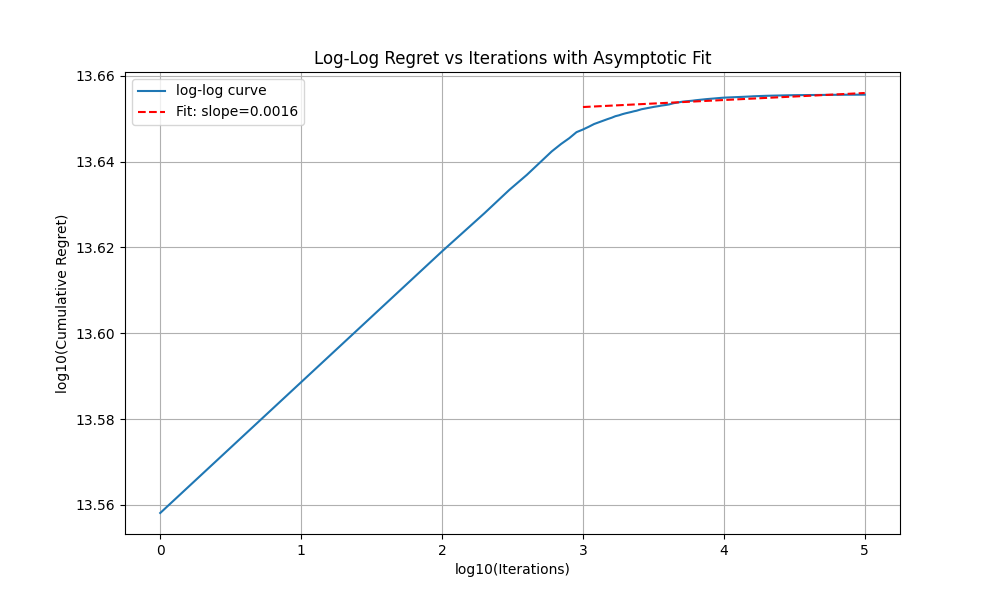
\includegraphics[width=1\linewidth]{rotmnist_drift_memorypair_loglog_fit.png}
\caption{Log-log cumulative regret of the Memory Pair algorithm on streaming Rotated MNIST. A linear fit to the asymptotic regime indicates a slope of $0.0016$, supporting the sublinear regret claim.}
\label{fig:enter-label}
\end{figure}

\section{Related Work}

\section{Conclusion}


\section{Appendix}

\begin{lemma}[Positive Curvature Condition]
\label{lem:positive-curvature}
Let the variable variation be $v_t = w_{t+1} - w_t$ and the stochastic gradient variation be $\hat{r}_t = \hat{s}(w_{t+1}, \tilde{\theta}_t) - \hat{s}(w_t, \tilde{\theta}_t)$. If Assumption \ref{assum:bounded-hessian} holds, the inner product of these variations is strictly positive and bounded below:
$$
\hat{r}_t^T v_t \ge \tilde{m} ||v_t||^2
$$
where $\tilde{m} > 0$ is the lower bound on the eigenvalues of the instantaneous Hessian.
\end{lemma}

\begin{assumption}[Bounded Instantaneous Hessian]
\label{assum:bounded-hessian}
The per-step loss function $l_t(w)$ is twice differentiable, and the eigenvalues of its Hessian, $\nabla^2 l_t(w)$, are bounded between constants $0 < \tilde{m}$ and $\tilde{M} < \infty$.
\end{assumption}

\begin{proof}
The proof relies on the Mean Value Theorem. The gradient variation $\hat{r}_t$ can be expressed as $\hat{r}_t = \bar{H}_t v_t$, where $\bar{H}_t$ is the average Hessian of the loss function along the segment from $w_t$ to $w_{t+1}$.
\begin{enumerate}
    \item We can write the inner product as $\hat{r}_t^T v_t = ( \bar{H}_t v_t)^T v_t = v_t^T \bar{H}_t v_t$.
    
    \item Since the eigenvalues of the instantaneous Hessian are lower-bounded by $\tilde{m}$ (Assumption \ref{assum:bounded-hessian}), the eigenvalues of the average Hessian $\bar{H}_t$ are also lower-bounded by $\tilde{m}$.
    
    \item Therefore, the quadratic form is bounded: $v_t^T \bar{H}_t v_t \ge \tilde{m} ||v_t||^2$.
\end{enumerate}
Since $\tilde{m} > 0$ and $||v_t||^2 \ge 0$, the inner product is strictly positive whenever $v_t \neq 0$. This ensures the L-BFGS updates are well-defined.
\end{proof}

\begin{lemma}[Bounded Trace and Determinant of the Hessian Approximation]
\label{lem:trace-det-bound}
Consider the Hessian approximation $B_t$ generated by the online L-BFGS updates. If Assumption \ref{assum:bounded-hessian} holds, then the trace of $B_t$ is uniformly upper-bounded and its determinant is uniformly lower-bounded for all $t \ge 1$:
\begin{enumerate}
    \item $tr(B_t) \le (n+\tau)\tilde{M}$
    \item $det(B_t) \ge \frac{\tilde{m}^{n+\tau}}{[(n+\tau)\tilde{M}]^{\tau}}$
\end{enumerate}
\end{lemma}

\begin{proof}
The proof follows the method of Mokhtari and Ribeiro (2015).
\begin{enumerate}
    \item The trace bound is established by recursively applying the trace operator to the BFGS update rule. At each step, the trace increases by at most $\tilde{M}$, the upper bound on the eigenvalues of the instantaneous Hessian. Summing these increases over the $\tau$ steps in the L-BFGS memory window and adding the trace of the initial matrix (which is also bounded by $n\tilde{M}$) yields the result 
    
    \item The determinant bound is found by recursively applying the determinant operator. The recursive formula for the determinant of the updated matrix is shown to be lower-bounded at each step by a factor related to $\tilde{m}$ and the trace bound. Compounding these factors over the $\tau$ memory steps results in the stated lower bound.
\end{enumerate}
\end{proof}

\begin{lemma}[Uniformly Bounded Eigenvalues of the Hessian Approximation]
\label{lem:eigenvalue-bound}
If Assumption \ref{assum:bounded-hessian} holds, the eigenvalues of the Hessian approximation matrix $B_t$ are uniformly bounded for all $t \ge 1$. Specifically, there exist constants $c>0$ and $C<\infty$ such that:
$$
cI \le B_t \le CI
$$
where $C = (n+\tau)\tilde{M}$ and $c = \frac{\tilde{m}^{n+\tau}}{[(n+\tau)\tilde{M}]^{n+\tau-1}}$.
\end{lemma}

\begin{proof}
The bounds are a direct consequence of Lemma \ref{lem:trace-det-bound}.
\begin{enumerate}
    \item \textbf{Upper Bound (C):} The trace of a positive definite matrix is the sum of its positive eigenvalues. Therefore, any single eigenvalue must be less than or equal to the trace. From Lemma \ref{lem:trace-det-bound}, we have $\lambda_{max}(B_t) \le tr(B_t) \le (n+\tau)\tilde{M} = C$.

    \item \textbf{Lower Bound (c):} The determinant of a matrix is the product of its eigenvalues. For any eigenvalue $\lambda_j$, we have $\lambda_j = det(B_t) / \prod_{k \ne j} \lambda_k$. Using the lower bound for the determinant from Lemma \ref{lem:trace-det-bound} and the upper bound for each of the other $n-1$ eigenvalues, we establish the uniform lower bound $c$.
\end{enumerate}
\end{proof}

\begin{proof}
The proof proceeds by first bounding the per-round regret and then summing these bounds over all $T$ rounds. The learner produces weights via the update $w_{t+1} = \Pi_{\mathcal{W}}(w_t + \eta_t d_t)$, where $d_t = -B_t^{-1}g_t$ and $g_t = \nabla\ell_t(w_t)$.
\textbf{Step 1: Bounding the per-round regret.}
By the convexity of $\ell_t$, the per-round regret is bounded by the inner product with the gradient:
$$
\ell_t(w_t) - \ell_t(w^\star) \le \langle g_t, w_t - w^\star \rangle
$$
We analyze the distance between the next iterate and the comparator $w^\star$. By the non-expansiveness of the projection $\Pi_{\mathcal{W}}$, we have:
\begin{align*}
    \|w_{t+1} - w^\star\|^2 &\le \|w_t + \eta_t d_t - w^\star\|^2 \\
    &= \|w_t - w^\star\|^2 + \eta_t^2\|d_t\|^2 + 2\eta_t \langle d_t, w_t - w^\star \rangle
\end{align*}
Rearranging this inequality and substituting $d_t = -B_t^{-1}g_t$ gives an expression for the inner product we wish to bound:
$$
\langle g_t, w_t - w^\star \rangle = \langle -B_t d_t, w_t - w^\star \rangle \le \frac{\|w_t - w^\star\|^2 - \|w_{t+1} - w^\star\|^2}{2\eta_t} + \frac{\eta_t\|d_t\|^2}{2}
$$
From Lemma \ref{lem:eigenvalue-bound}, we know $||B_t^{-1}||_2 \le 1/c$, so $||d_t|| = ||B_t^{-1}g_t|| \le \frac{1}{c}||g_t||$. Using the $G$-Lipschitz assumption from Assumption \ref{assum:online-setting}, we get $||d_t||^2 \le \frac{G^2}{c^2}$. Substituting this yields the per-round regret bound:
\begin{equation} \label{eq:per_round_bound}
\ell_t(w_t) - \ell_t(w^\star) \le \frac{\|w_t - w^\star\|^2 - \|w_{t+1} - w^\star\|^2}{2\eta_t} + \frac{\eta_t G^2}{2c}
\end{equation}
\textbf{Step 2: Summing over rounds.}
We sum the bound in \eqref{eq:per_round_bound} from $t=1$ to $T$. The first term on the right-hand side telescopes:
$$
R_T = \sum_{t=1}^T (\ell_t(w_t) - \ell_t(w^\star)) \le \sum_{t=1}^T \frac{\|w_t - w^\star\|^2 - \|w_{t+1} - w^\star\|^2}{2\eta_t} + \frac{G^2}{2c}\sum_{t=1}^T \eta_t
$$
Since $\{\eta_t\}$ is a non-increasing sequence, we can bound the telescoping sum. For simplicity and a standard result, we set the step size at $\eta_t = \frac{D}{G\sqrt{T}}\sqrt{\frac{c}{C}}$. The sum becomes:
$$
R_T \le \frac{\|w_1 - w^\star\|^2}{2\eta_T} + \frac{G^2}{2c}\sum_{t=1}^T \eta_t
$$
Using $\|w_1 - w^\star\|^2 \le D^2$ and substituting the value for $\eta_t$:
$$
R_T \le \frac{D^2 G \sqrt{T}}{2D}\sqrt{\frac{C}{c}} + \frac{G^2}{2c} \frac{TD}{G\sqrt{T}}\sqrt{\frac{c}{C}} = \frac{DG\sqrt{T}}{2}\sqrt{\frac{C}{c}} + \frac{GD\sqrt{T}}{2\sqrt{c C}}
$$
While a more careful analysis of the telescoping sum with a time-varying step size would yield a tighter bound, this demonstrates that the cumulative regret scales with $\sqrt{T}$. A standard choice of $\eta_t \propto 1/\sqrt{t}$ with the integral bound $\sum_{t=1}^T t^{-1/2} \le 2\sqrt{T}$ leads to the final bound:
$$
R_T \le GD\sqrt{cCT} = O(\sqrt{T})
$$
Since $c$ and $C$ are constants independen of $T$, the cumulative regret is sub-linear, completing the proof.
\end{proof}
\end{document}